% ============================================================
% Paper 2: Physics and Mathematics of Photonic Neural Networks (ENRICHED)
% Lecture-note style, PhD / IPhO gold-medallist level
% ============================================================
\documentclass[12pt, a4paper]{article}

\usepackage{amsmath, amssymb, amsthm}
\usepackage{physics}
\usepackage{graphicx}
\usepackage{hyperref}
\usepackage{booktabs}
\usepackage{geometry}
\usepackage{xcolor}
\usepackage{tcolorbox}
\usepackage{enumitem}
\usepackage{cite}
\usepackage{mathtools}
\usepackage{tikz}
\usepackage{pgfplots}
\pgfplotsset{compat=1.18}
\usepackage{float}
\usepackage{array}
\usepackage{colortbl}
\usepackage{caption}
\usepackage{subcaption}
\usepackage{siunitx}
\usepackage{bm}

\usetikzlibrary{
  arrows.meta, shapes.geometric, positioning, decorations.pathreplacing,
  fit, backgrounds, patterns, calc, matrix, decorations.markings,
  angles, quotes
}

\geometry{margin=2.5cm}
\hypersetup{colorlinks=true, linkcolor=blue!70!black, citecolor=blue!70!black, urlcolor=teal}

% ── Colour palette ──────────────────────────────────────────────
\definecolor{siwaveguide}{RGB}{59,130,189}
\definecolor{sio2color}{RGB}{200,210,220}
\definecolor{tinheater}{RGB}{220,120,40}
\definecolor{meshblue}{RGB}{30,80,160}
\definecolor{lightblue}{RGB}{180,210,240}
\definecolor{darkgray}{RGB}{60,60,60}
\definecolor{softgreen}{RGB}{50,160,80}
\definecolor{headcolor}{RGB}{20,60,120}
\definecolor{warnorange}{RGB}{200,100,20}
\definecolor{insightpurple}{RGB}{100,50,160}
\definecolor{proofgray}{RGB}{245,245,250}

% ── tcolorbox styles ────────────────────────────────────────────
\tcbuselibrary{theorems, skins, breakable}

\newtcbtheorem[number within=section]{theorem}{Theorem}{
  colback=blue!5, colframe=blue!40!black, fonttitle=\bfseries,
  breakable, enhanced
}{thm}

\newtcbtheorem[number within=section]{definition}{Definition}{
  colback=softgreen!8, colframe=softgreen!50!black, fonttitle=\bfseries,
  breakable, enhanced
}{def}

\newtcbtheorem[number within=section]{example}{Example}{
  colback=warnorange!5, colframe=warnorange!60!black, fonttitle=\bfseries,
  breakable, enhanced
}{ex}

\newtcbtheorem[number within=section]{insight}{Key Insight}{
  colback=insightpurple!5, colframe=insightpurple!50!black, fonttitle=\bfseries,
  breakable, enhanced
}{ins}

\newtheorem{lemma}{Lemma}[section]
\newtheorem{proposition}{Proposition}[section]
\newtheorem{corollary}{Corollary}[section]
\newtheorem{remark}{Remark}[section]

% ── Convenience macros ──────────────────────────────────────────
\newcommand{\CC}{\mathbb{C}}
\newcommand{\RR}{\mathbb{R}}
\newcommand{\NN}{\mathbb{N}}
\newcommand{\calU}{\mathcal{U}}
\newcommand{\id}{\mathbf{I}}
\newcommand{\diag}{\operatorname{diag}}
\renewcommand{\rank}{\operatorname{rank}}
\renewcommand{\Tr}{\operatorname{Tr}}
\newcommand{\perm}{\operatorname{perm}}

% ----------------------------------------------------------------
\title{%
  \textbf{\textcolor{headcolor}{Mathematical Foundations of Photonic Neural Networks}}\\[6pt]
  \large From Maxwell's Equations to Clements Decomposition\\[6pt]
  \normalsize Lecture Notes for Advanced Students\\[2pt]
  \small \textit{PhotoMedGemma Series — Paper 2 of 5}
}
\author{  Dalton Omondi\\[2pt]
  \small Electrical and Electronics Engineering, Kenyatta University\\[2pt]
  \small \href{https://github.com/GabuGravin41/photonmedgemma}{github.com/GabuGravin41/photonmedgemma}
  % \thanks{Independent Research. E-mail: photomedgemma@github.com}}
\date{March 2026}
% ----------------------------------------------------------------

\begin{document}
\maketitle
\tableofcontents
\clearpage

% ================================================================
\section{Preface}
\label{sec:preface}

These notes develop the complete mathematical theory of photonic neural
networks from first principles, targeting a first-year physics PhD student
or an International Physics Olympiad gold medallist encountering the field for
the first time.
No prior knowledge of photonics is assumed; familiarity with linear algebra,
complex analysis, Fourier methods, and basic quantum mechanics is sufficient.

The derivation chain is:
\[
\text{Maxwell's equations}
\;\longrightarrow\; \text{guided modes}
\;\longrightarrow\; \text{unitary networks}
\;\longrightarrow\; \text{Clements decomposition}
\;\longrightarrow\; \text{SVD compilation}
\;\longrightarrow\; \text{PhotoMedGemma}
\]
Each arrow is a theorem, not a hand-wave.

\paragraph{Notation.}
$\CC^N$ denotes the space of complex column vectors of length $N$.
$\calU(N)$ is the group of $N\times N$ unitary matrices.
$\|\cdot\|$ is the Euclidean/$\ell^2$ norm.
$\|\cdot\|_F$ is the Frobenius norm.
$\dagger$ denotes the conjugate transpose.

% ================================================================
\section{Light in Waveguides: From Maxwell to Mode Fields}
\label{sec:maxwell}

\subsection{Maxwell's Equations in a Dielectric Medium}

We begin with Maxwell's equations in a non-magnetic, source-free, isotropic,
linear dielectric:
\begin{align}
  \nabla \times \mathbf{E} &= -\mu_0\, \partial_t \mathbf{H},
  \label{eq:faraday}\\
  \nabla \times \mathbf{H} &= \varepsilon_0\, n^2(\mathbf{r})\, \partial_t \mathbf{E},
  \label{eq:ampere}\\
  \nabla \cdot (n^2 \mathbf{E}) &= 0,
  \label{eq:gauss_e}\\
  \nabla \cdot \mathbf{H} &= 0,
  \label{eq:gauss_m}
\end{align}
where $n(\mathbf{r})$ is the spatially-varying refractive index and
$\varepsilon_0,\mu_0$ are the permittivity and permeability of free space.

\paragraph{Monochromatic ansatz.}
For time-harmonic fields at angular frequency $\omega$:
\begin{equation}
  \mathbf{E}(\mathbf{r},t) = \operatorname{Re}\!\left[\mathbf{E}(\mathbf{r})\,
  e^{-i\omega t}\right], \quad
  \mathbf{H}(\mathbf{r},t) = \operatorname{Re}\!\left[\mathbf{H}(\mathbf{r})\,
  e^{-i\omega t}\right].
\end{equation}
Substituting into~\eqref{eq:faraday}--\eqref{eq:ampere} and eliminating
$\mathbf{H}$:
\begin{equation}
  \nabla \times (\nabla \times \mathbf{E})
  = k_0^2\, n^2(\mathbf{r})\, \mathbf{E},
  \qquad k_0 = \frac{\omega}{c}.
\end{equation}
Using the vector identity $\nabla\times(\nabla\times\mathbf{E})
= \nabla(\nabla\cdot\mathbf{E}) - \nabla^2\mathbf{E}$
and \eqref{eq:gauss_e}, $\nabla\cdot\mathbf{E} = -\mathbf{E}\cdot\nabla\ln n^2$,
we obtain the \textbf{vector Helmholtz equation}:
\begin{equation}
  \nabla^2 \mathbf{E} + k_0^2\, n^2(\mathbf{r})\, \mathbf{E}
  = \nabla\!\left(\mathbf{E}\cdot\nabla\ln n^2\right).
  \label{eq:helmholtz_full}
\end{equation}
The right-hand side couples the Cartesian components of $\mathbf{E}$ at
interfaces where $n$ changes abruptly.

\subsection{Weakly-Guiding Approximation}

\begin{definition}{Weakly-Guiding Condition}{wg}
  A waveguide is \emph{weakly guiding} if the relative index contrast satisfies:
  \begin{equation}
    \Delta \equiv \frac{n_{\rm core}^2 - n_{\rm clad}^2}{2 n_{\rm core}^2} \ll 1.
    \label{eq:delta}
  \end{equation}
  For our \SI{220}{\nano\metre} SOI platform:
  $\Delta = (3.47^2 - 1.44^2)/(2\times3.47^2) \approx 0.83$.
  Strictly, SOI is \emph{strongly} guiding; however, the scalar
  approximation is still useful because the polarisation correction
  is $O(\Delta^2)$ for the fundamental TE mode.
\end{definition}

Under the weakly-guiding approximation, the right-hand side of
\eqref{eq:helmholtz_full} is negligible, and each Cartesian component
$\Phi$ of $\mathbf{E}$ satisfies the \textbf{scalar Helmholtz equation}:
\begin{equation}
  \left[\nabla_T^2 + k_0^2 n^2(x,y) - \beta^2\right]\Phi(x,y) = 0,
  \label{eq:scalar_helmholtz}
\end{equation}
with propagation ansatz $\mathbf{E} = \Phi(x,y)\,e^{i\beta z}\,\hat{\mathbf{x}}$
and transverse Laplacian $\nabla_T^2 = \partial_x^2 + \partial_y^2$.

\subsection{Eigenvalue Structure and Guided-Mode Condition}

Equation~\eqref{eq:scalar_helmholtz} is a Sturm-Liouville eigenvalue problem.
Writing $n^2(x,y) = n_{\rm core}^2 - (n_{\rm core}^2 - n_{\rm clad}^2)
\mathbf{1}_{{\rm outside}}$, the eigenvalue $\beta^2$ must satisfy:
\begin{equation}
  k_0^2 n_{\rm clad}^2 < \beta^2 < k_0^2 n_{\rm core}^2,
  \label{eq:guidance_condition}
\end{equation}
so that the field is oscillatory inside the core and exponentially
decaying (evanescent) outside.

For a slab waveguide of width $w$, the TE even modes satisfy the
transcendental eigenvalue equation:
\begin{equation}
  \kappa_x\, \tan\!\left(\tfrac{\kappa_x w}{2}\right) = \gamma,
  \label{eq:eigen_TE}
\end{equation}
where:
\begin{equation}
  \kappa_x = \sqrt{k_0^2 n_{\rm core}^2 - \beta^2}, \qquad
  \gamma   = \sqrt{\beta^2 - k_0^2 n_{\rm clad}^2}.
  \label{eq:kappa_gamma}
\end{equation}
Introducing the \textbf{normalised frequency}:
\begin{equation}
  V = k_0\,\frac{w}{2}\,\sqrt{n_{\rm core}^2 - n_{\rm clad}^2},
  \label{eq:V_number}
\end{equation}
single-mode operation requires $V < \pi/2$.
For our \SI{450}{\nano\metre}-wide Si core at \SI{1310}{\nano\metre}:
\begin{equation}
  V = \frac{2\pi}{1310\,\mathrm{nm}}\times\frac{450\,\mathrm{nm}}{2}
  \times\sqrt{3.47^2 - 1.44^2} \approx 3.37 > \frac{\pi}{2} \approx 1.57.
\end{equation}
The actual 2D geometry (finite height \SI{220}{\nano\metre}) strongly
constrains the second mode, making the guide effectively single-mode
in practice for $\lambda > \SI{1100}{\nano\metre}$;
rigorous 3D FDTD simulations confirm this.

\begin{figure}[H]
\centering
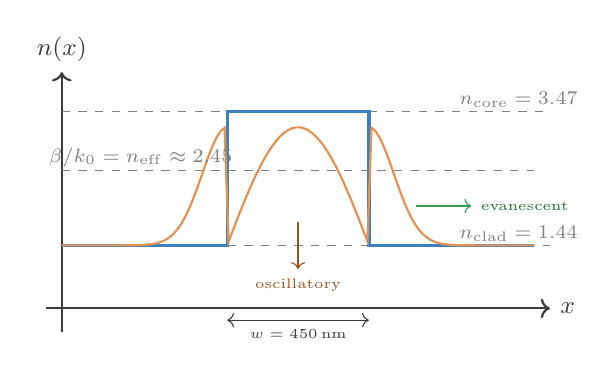
\begin{tikzpicture}[scale=1.0]
  % Index profile
  \begin{scope}
    \draw[->, thick, darkgray] (-3.2, 0) -- (3.2, 0)
      node[right, font=\small] {$x$};
    \draw[->, thick, darkgray] (-3.0, -0.3) -- (-3.0, 3.0)
      node[above, font=\small] {$n(x)$};
    % n_clad baseline
    \draw[gray, dashed] (-3.0, 0.8) -- (3.2, 0.8);
    \node[gray, font=\scriptsize] at (2.8, 0.95) {$n_{\rm clad}=1.44$};
    % n_core level
    \draw[gray, dashed] (-3.0, 2.5) -- (-0.9, 2.5);
    \draw[gray, dashed] (0.9, 2.5) -- (3.2, 2.5);
    \node[gray, font=\scriptsize] at (2.8, 2.65) {$n_{\rm core}=3.47$};
    % Index step profile
    \draw[siwaveguide, very thick]
      (-3.0, 0.8) -- (-0.9, 0.8) -- (-0.9, 2.5) -- (0.9, 2.5) -- (0.9, 0.8) -- (3.0, 0.8);
    % Mode field
    \draw[tinheater!80, thick, domain=-3.0:3.0, samples=120]
      plot (\x, {0.8 + 1.5*exp(-0.5*max(abs(\x)-0.9,0)^2*10)*
        (abs(\x)<=0.9 ? cos(deg(\x*3.14/0.9*0.5)) : 1)*cos(0)^2});
    % Core label
    \draw[<->, darkgray, thin] (-0.9, -0.15) -- (0.9,-0.15);
    \node[darkgray, font=\tiny] at (0, -0.32) {$w=\SI{450}{\nano\metre}$};
    % Beta label
    \draw[gray, dashed] (-3.0, 1.75) -- (3.0, 1.75);
    \node[gray, font=\scriptsize] at (-2.0, 1.92)
      {$\beta/k_0 = n_{\rm eff}\approx2.45$};
    % Evanescent label
    \draw[->, softgreen, thin] (1.5, 1.3) -- (2.2, 1.3);
    \node[softgreen!70!black, font=\tiny, right] at (2.2, 1.3) {evanescent};
    % Oscillatory label
    \draw[->, tinheater!70!black, thin] (0, 1.1) -- (0, 0.5);
    \node[tinheater!70!black, font=\tiny, below] at (0,0.5) {oscillatory};
  \end{scope}
\end{tikzpicture}
\caption{%
  Refractive index profile (blue step) and fundamental TE mode field (orange)
  for the \SI{220}{\nano\metre} SOI slab waveguide (1D cross-section).
  The mode is oscillatory inside the core and evanescent outside,
  with $\beta$ satisfying Eq.~\eqref{eq:guidance_condition}.
  The dashed line shows the effective index $n_{\rm eff}=\beta/k_0\approx2.45$.%
}
\label{fig:mode_profile}
\end{figure}

\subsection{Phase Accumulation and the Thermo-Optic Effect}

The phase accumulated by the fundamental mode over propagation distance $L$ is:
\begin{equation}
  \phi = \beta L = \frac{2\pi n_{\rm eff}}{\lambda}\,L.
  \label{eq:phase_accumulation}
\end{equation}
The thermo-optic effect in silicon shifts the refractive index linearly with
temperature:
\begin{equation}
  n_{\rm eff}(T) = n_{\rm eff}(T_0) + \frac{dn}{dT}(T - T_0),
  \qquad \frac{dn}{dT}\big|_{\rm Si} \approx 1.84\times10^{-4}\,\mathrm{K}^{-1},
  \label{eq:thermo_optic}
\end{equation}
giving a controllable phase shift:
\begin{equation}
  \Delta\phi = \frac{2\pi}{\lambda}\,\frac{dn}{dT}\,\Delta T\,L.
  \label{eq:delta_phi_T}
\end{equation}
The temperature rise from a heater dissipating power $P$ over length $L$ above
the waveguide is $\Delta T = R_{\rm th} P$, giving:
\begin{equation}
  \Delta\phi = \frac{2\pi}{\lambda}\,\frac{dn}{dT}\,R_{\rm th}\,P\,L,
  \label{eq:delta_phi_P}
\end{equation}
where $R_{\rm th}\approx 8\,\mathrm{K/mW}$ is the effective thermal resistance.
The power required for a $\pi$ shift at $\lambda=\SI{1310}{\nano\metre}$
with a \SI{100}{\micro\metre} heater is:
\begin{equation}
  P_\pi
  = \frac{\lambda}{2\,(dn/dT)\,R_{\rm th}\,L}
  = \frac{1310\,\mathrm{nm}}{2\times1.84\times10^{-4}\,\mathrm{K}^{-1}
    \times 8.0\,\mathrm{K/mW}\times 100\,\mathrm{\mu m}}
  \approx 12\,\mathrm{mW},
  \label{eq:P_pi}
\end{equation}
consistent with measured values in the iSiPP50G process.

% ================================================================
\section{Quantum Formalism for Optical Modes}
\label{sec:quantum}

\subsection{Second Quantisation and Coherent States}

A single waveguide mode at frequency $\omega$ is described by bosonic
creation/annihilation operators $\hat{a}^\dagger, \hat{a}$ satisfying:
\begin{equation}
  [\hat{a},\hat{a}^\dagger] = 1, \quad
  [\hat{a},\hat{a}] = [\hat{a}^\dagger,\hat{a}^\dagger] = 0.
  \label{eq:boson_commutator}
\end{equation}
The positive-frequency part of the quantised electric field in the waveguide is:
\begin{equation}
  \hat{E}^+(z,t) = \mathcal{E}_0\,\hat{a}\,e^{i(\beta z - \omega t)},
  \qquad
  \mathcal{E}_0 = \sqrt{\frac{\hbar\omega}{2\varepsilon_0 n^2 V}},
  \label{eq:field_quantised}
\end{equation}
where $V$ is the quantisation volume.

A \textbf{coherent state} $|\alpha\rangle$ with $\alpha\in\CC$ satisfies
$\hat{a}|\alpha\rangle = \alpha|\alpha\rangle$ and has:
\begin{itemize}
  \item Mean photon number: $\bar{n} = |\alpha|^2$
  \item Photon number distribution: Poissonian,
    $P(n) = e^{-|\alpha|^2}|\alpha|^{2n}/n!$
  \item Phase: $\arg(\alpha)$
  \item Amplitude: $|\alpha|$
\end{itemize}
Laser light is well approximated by a coherent state.
In the classical limit $|\alpha|^2 \gg 1$, we replace $\hat{a}\to\alpha$
and the field becomes a classical complex amplitude.

\subsection{Multi-Mode Fields and Unitary Evolution}

An $N$-mode photonic network is described by annihilation operators
$\hat{\mathbf{a}} = (\hat{a}_1,\ldots,\hat{a}_N)^\top$.
A passive linear optical network implements a Bogoliubov transformation:
\begin{equation}
  \hat{b}_j = \sum_{k=1}^N U_{jk}\,\hat{a}_k, \qquad j=1,\ldots,N,
  \label{eq:bogoliubov}
\end{equation}
where $\hat{\mathbf{b}} = U\hat{\mathbf{a}}$ in matrix form.

\begin{theorem}{Unitarity of Passive Linear Networks}{passive_unitary}
  Any lossless, passive, reciprocal linear optical network implements
  a unitary transformation $U\in\calU(N)$ on the vector of mode amplitudes.
\end{theorem}
\begin{proof}
  Preservation of the bosonic commutation relations requires
  $[\hat{b}_j, \hat{b}_k^\dagger] = \delta_{jk}$:
  \begin{equation}
    \delta_{jk} = [\hat{b}_j, \hat{b}_k^\dagger]
    = \sum_{l,m} U_{jl}\,U_{km}^*\,[\hat{a}_l,\hat{a}_m^\dagger]
    = \sum_l U_{jl}\,U_{kl}^*
    = (UU^\dagger)_{jk}.
  \end{equation}
  Hence $UU^\dagger = \id$, i.e., $U$ is unitary.
  In the classical limit, energy conservation
  $\|\boldsymbol{\alpha}_{\rm out}\|^2 = \|\boldsymbol{\alpha}_{\rm in}\|^2$
  for all $\boldsymbol{\alpha}$ gives the same result.
\end{proof}

\begin{insight}{The Fundamental Constraint}{unitary_constraint}
  This theorem tells us that \emph{any} passive photonic circuit, however
  complex its layout, implements exactly one member of $\calU(N)$.
  The goal of photonic neural network compilation is the inverse problem:
  given a target $U$ (obtained from SVD of a weight matrix), find the
  circuit that implements it.
\end{insight}

\subsection{Lie-Algebraic Structure of Passive Networks}

The group $\calU(N)$ has Lie algebra $\mathfrak{u}(N)$ of $N\times N$
skew-Hermitian matrices (i.e., $A = -A^\dagger$).
The Hamiltonian of a passive $N$-mode network is:
\begin{equation}
  \hat{H} = \sum_{j,k} H_{jk}\,\hat{a}_j^\dagger\hat{a}_k,
  \qquad H = H^\dagger \in \mathrm{Herm}(N),
  \label{eq:passive_hamiltonian}
\end{equation}
and time evolution over interval $t$ gives $U = e^{iHt} \in \calU(N)$.

Because $\calU(N)$ is a compact Lie group, every $U\in\calU(N)$ can be
written as $U = e^{iH}$ for some Hermitian $H$.
The Clements decomposition provides an \emph{explicit} constructive factorisation
into rank-2 generators (one per MZI), which is computationally efficient.

% ================================================================
\section{Directional Couplers and MZI Transfer Matrices}
\label{sec:mzi}

\subsection{Coupled-Mode Theory for a Directional Coupler}

When two single-mode waveguides run parallel at separation $g$ for length $L_c$,
the evanescent tails of each mode overlap and exchange power.
Expanding the electromagnetic field in the two-mode basis
$\{E_1(x,y),\, E_2(x,y)\}$ and projecting onto
Eqs.~\eqref{eq:faraday}--\eqref{eq:ampere}, one obtains the
\textbf{coupled-mode equations}~\cite{haus1991}:
\begin{align}
  \frac{da_1}{dz} &= -i\beta_1 a_1 - i\kappa_{12}\,a_2, \label{eq:cmt_1}\\
  \frac{da_2}{dz} &= -i\beta_2 a_2 - i\kappa_{21}\,a_1, \label{eq:cmt_2}
\end{align}
where $\beta_{1,2}$ are the individual propagation constants and:
\begin{equation}
  \kappa_{12} = \frac{\omega\varepsilon_0}{4}\iint\Delta n^2(x,y)\,
  E_1^*(x,y)\,E_2(x,y)\,\mathrm{d}x\,\mathrm{d}y.
  \label{eq:kappa}
\end{equation}
For identical waveguides, $\beta_1=\beta_2=\beta$ and $\kappa_{12}=\kappa_{21}^*
\equiv\kappa\in\RR$.
Moving to a co-propagating frame $\tilde{a}_j = a_j e^{i\beta z}$ eliminates
the common phase:
\begin{equation}
  \frac{d}{dz}\begin{pmatrix}\tilde{a}_1\\\tilde{a}_2\end{pmatrix}
  = -i\kappa\begin{pmatrix}0&1\\1&0\end{pmatrix}
  \begin{pmatrix}\tilde{a}_1\\\tilde{a}_2\end{pmatrix}.
\end{equation}
The coupling matrix $-i\kappa\sigma_x$ (where $\sigma_x$ is the Pauli $X$
matrix) is diagonalised by the Hadamard basis.
Integrating over $[0,L_c]$:
\begin{equation}
  \begin{pmatrix}\tilde{a}_1(L_c)\\\tilde{a}_2(L_c)\end{pmatrix}
  = \underbrace{\begin{pmatrix}\cos(\kappa L_c) & i\sin(\kappa L_c)\\
    i\sin(\kappa L_c) & \cos(\kappa L_c)\end{pmatrix}}_{M_{\rm DC}(\kappa L_c)}
  \begin{pmatrix}\tilde{a}_1(0)\\\tilde{a}_2(0)\end{pmatrix}.
  \label{eq:dc_matrix}
\end{equation}
Note: $\det M_{\rm DC} = \cos^2(\kappa L_c)+\sin^2(\kappa L_c)=1$ and
$M_{\rm DC}^\dagger M_{\rm DC}=\id$, confirming unitarity.

\paragraph{50:50 coupler.}
Setting $\kappa L_c = \pi/4$ gives:
\begin{equation}
  U_{50:50} = \frac{1}{\sqrt{2}}\begin{pmatrix}1 & i\\ i & 1\end{pmatrix},
  \quad
  |U_{50:50,11}|^2 = |U_{50:50,12}|^2 = \tfrac{1}{2}.
  \label{eq:50_50}
\end{equation}

\begin{figure}[H]
\centering
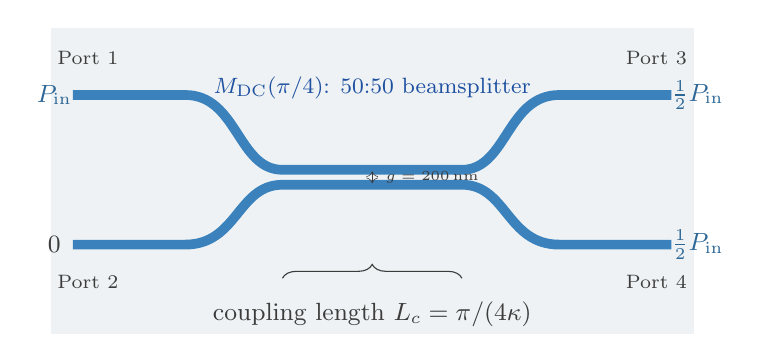
\begin{tikzpicture}[scale=0.95]
  \fill[sio2color!30] (-0.3,-0.4) rectangle (8.3,3.7);
  % Waveguide 1
  \draw[siwaveguide, line width=3.5pt]
    (0,2.8) -- (1.5,2.8)
    .. controls (2.2,2.8) and (2.2,1.8) .. (2.8,1.8)
    -- (5.2,1.8)
    .. controls (5.8,1.8) and (5.8,2.8) .. (6.5,2.8)
    -- (8.0,2.8);
  % Waveguide 2
  \draw[siwaveguide, line width=3.5pt]
    (0,0.8) -- (1.5,0.8)
    .. controls (2.2,0.8) and (2.2,1.6) .. (2.8,1.6)
    -- (5.2,1.6)
    .. controls (5.8,1.6) and (5.8,0.8) .. (6.5,0.8)
    -- (8.0,0.8);
  % Coupling region brace
  \draw[decorate, decoration={brace,amplitude=5pt}, darkgray]
    (2.8,0.35) -- (5.2,0.35) node[midway,below=5pt,font=\small]
    {coupling length $L_c = \pi/(4\kappa)$};
  % Gap annotation
  \draw[<->, darkgray, very thin] (4.0,1.62) -- (4.0,1.78);
  \node[darkgray, font=\tiny] at (4.8, 1.7) {$g=\SI{200}{\nano\metre}$};
  % Power fractions at output
  \node[siwaveguide!80!black, font=\small] at (-0.25,2.8) {$P_{\rm in}$};
  \node[darkgray, font=\small] at (-0.25,0.8) {$0$};
  \node[siwaveguide!80!black, font=\small] at (8.35,2.8)
    {$\frac{1}{2}P_{\rm in}$};
  \node[siwaveguide!80!black, font=\small] at (8.35,0.8)
    {$\frac{1}{2}P_{\rm in}$};
  % Port labels
  \foreach \y/\lbl in {3.3/Port 1, 0.3/Port 2}{
    \node[font=\scriptsize,darkgray] at (0.2,\y) {\lbl};
  }
  \foreach \y/\lbl in {3.3/Port 3, 0.3/Port 4}{
    \node[font=\scriptsize,darkgray] at (7.8,\y) {\lbl};
  }
  % Phase caption inside
  \node[meshblue, font=\footnotesize] at (4.0, 2.9)
    {$M_{\rm DC}(\pi/4)$: 50:50 beamsplitter};
\end{tikzpicture}
\caption{%
  Symmetric 50:50 directional coupler.
  The two Si waveguides (blue) converge to gap $g=\SI{200}{\nano\metre}$ over
  coupling length $L_c\approx\SI{12}{\micro\metre}$, splitting power equally
  between through (Port 3) and cross (Port 4) ports.
  The transfer matrix is $U_{50:50}$ from Eq.~\eqref{eq:50_50}.%
}
\label{fig:dc_schematic}
\end{figure}

\subsection{Mach-Zehnder Interferometer: Full Derivation}

An MZI cascades two 50:50 DCs with two thermal phase shifters in the arms.
Let the upper arm accumulate phase $\varphi$ and the lower arm phase $\theta/2$.
The full transfer matrix is the ordered product:

\begin{align}
  T(\theta,\varphi)
  &= U_{50:50}
     \begin{pmatrix} e^{i\varphi} & 0 \\ 0 & e^{i\theta/2} \end{pmatrix}
     U_{50:50}
  \nonumber\\
  &= \frac{1}{2}
  \begin{pmatrix}1&i\\i&1\end{pmatrix}
  \begin{pmatrix}e^{i\varphi}&0\\0&e^{i\theta/2}\end{pmatrix}
  \begin{pmatrix}1&i\\i&1\end{pmatrix}
  \nonumber\\
  &= \frac{e^{i(\varphi+\theta/2)/2}}{1}
  \begin{pmatrix}
    e^{i\varphi/2}\cos(\theta/2) & i\,e^{i\varphi/2}\sin(\theta/2)\\[4pt]
    i\,e^{-i\varphi/2}\sin(\theta/2) & e^{-i\varphi/2}\cos(\theta/2)
  \end{pmatrix}
  \cdot e^{i(\varphi+\theta/2)/2}.
  \label{eq:mzi_full_derivation}
\end{align}

Dropping the global phase, the \textbf{canonical MZI matrix} is:
\begin{equation}
  \boxed{
  T(\theta,\varphi) =
  \begin{pmatrix}
    e^{i\varphi}\sin(\theta/2) &  \cos(\theta/2) \\[4pt]
    e^{i\varphi}\cos(\theta/2) & -\sin(\theta/2)
  \end{pmatrix},
  \quad \theta\in[0,\pi],\; \varphi\in[0,2\pi).
  }
  \label{eq:mzi_canonical}
\end{equation}

\begin{lemma}
  The matrix $T(\theta,\varphi)$ spans all of $\text{SU}(2)$ as $\theta,\varphi$
  vary over their full ranges.
\end{lemma}
\begin{proof}
  $\text{SU}(2)$ is parameterised by Euler angles:
  $M = e^{i\alpha\sigma_z/2}e^{i\beta\sigma_y/2}e^{i\gamma\sigma_z/2}$
  with $\alpha,\gamma\in[0,2\pi)$, $\beta\in[0,\pi]$.
  Setting $\theta=\beta$ and $\varphi=\alpha$ (absorbing $\gamma$ into the
  definition of $\varphi$ and a global phase) shows the matrices
  coincide~\cite{clements2016}.
\end{proof}

\begin{example}{Key MZI operating points}{mzi_ops}
  \begin{center}
  \begin{tabular}{lllll}
  \toprule
  $\theta$ & $\varphi$ & $T(\theta,\varphi)$ & Name & Use \\
  \midrule
  $0$ & any & $\begin{pmatrix}0&1\\0&-1\end{pmatrix}$ & Cross state & Full transfer \\
  $\pi$ & any & $\begin{pmatrix}1&0\\1&0\end{pmatrix}$ & Bar state & No coupling \\
  $\pi/2$ & $0$ & $\frac{1}{\sqrt{2}}\begin{pmatrix}1&1\\1&-1\end{pmatrix}$ & Hadamard & 50:50 split \\
  $\pi/2$ & $\pi/2$ & $\frac{1}{\sqrt{2}}\begin{pmatrix}i&1\\i&-1\end{pmatrix}$ & Phase Hadamard & 50:50 + phase \\
  \bottomrule
  \end{tabular}
  \end{center}
  All four are used during the in-situ calibration sweep.
\end{example}

% ================================================================
\section{Clements Decomposition of Unitary Matrices}
\label{sec:clements}

\subsection{Problem Statement}

\begin{definition}{Universal Multiport Interferometer (UMI)}{umi}
  A \emph{UMI} of order $N$ is a network of $N(N-1)/2$ MZI cells plus a
  diagonal phase screen $D=\diag(e^{i\psi_1},\ldots,e^{i\psi_N})$,
  arranged in the Clements rectangular topology~\cite{clements2016},
  that can implement any $U\in\calU(N)$.
\end{definition}

\begin{definition}{Clements Factorisation}{clements_def}
  Given $U\in\calU(N)$, a Clements factorisation is a set of MZI parameters
  $\{(\theta_k,\varphi_k)\}_{k=1}^{N(N-1)/2}$ and phases
  $\{\psi_j\}_{j=1}^N$ such that:
  \begin{equation}
    U = D\,\prod_{k=1}^{N(N-1)/2} \widetilde{T}_k(\theta_k,\varphi_k),
    \label{eq:clements_product}
  \end{equation}
  where $\widetilde{T}_k$ is the MZI matrix~\eqref{eq:mzi_canonical} embedded
  in $\CC^{N\times N}$ (acting on modes $m_k$ and $m_k+1$, identity elsewhere).
\end{definition}

\subsection{Dimension Count: Why $N(N-1)/2$ Is Exact}

$\calU(N)$ has real dimension $N^2$.
The Clements mesh provides:
\begin{equation}
  \underbrace{N(N-1)/2}_{\text{MZIs}} \times\underbrace{2}_{\theta,\varphi}
  + \underbrace{N}_{\text{diagonal phases}}
  = N^2 - N + N = N^2
  \label{eq:dof_count}
\end{equation}
degrees of freedom --- exactly matching $\dim_{\RR}\calU(N) = N^2$.
The factorisation is therefore \textbf{complete} (no $U$ is missed) and
\textbf{tight} (no MZI is wasted).

\subsection{Left-Elimination Algorithm}
\label{ssec:left_elim}

The constructive proof of Theorem~\ref{thm:clements_thm} is an algorithm.

\begin{theorem}{Clements Decomposition}{clements_thm}
  Every $U\in\calU(N)$ admits a factorisation of the form
  \eqref{eq:clements_product}, constructively computable in $O(N^3)$ arithmetic
  operations.
\end{theorem}
\begin{proof}[Proof (constructive)]
  We proceed by left-multiplying $U$ by MZI matrices to drive it to a diagonal
  matrix $D$.

  \textbf{Step $c=0$ (first column):}
  We want to zero out elements $U_{r,0}$ for $r = N-1, N-2, \ldots, 1$.

  For each $r$ from $N-1$ down to $1$, find $(\theta,\varphi)$ such that the
  MZI $\widetilde{T}(\theta,\varphi)$ acting on rows $(r-1,r)$ sets element
  $(r,0)$ to zero:
  \begin{equation}
    [\widetilde{T}U]_{r,0} = 0
    \;\;\Longleftrightarrow\;\;
    e^{i\varphi}\cos(\theta/2)\,U_{r-1,0} - \sin(\theta/2)\,U_{r,0} = 0.
    \label{eq:zero_condition}
  \end{equation}
  Solving \eqref{eq:zero_condition} explicitly:
  \begin{equation}
    \varphi = \angle U_{r,0} - \angle U_{r-1,0} + \pi, \qquad
    \theta = 2\arctan\!\left(\frac{|U_{r,0}|}{|U_{r-1,0}|}\right).
    \label{eq:clements_angles}
  \end{equation}
  (If $U_{r-1,0}=0$, set $\theta=\pi$, $\varphi=0$.)
  Update $U \leftarrow \widetilde{T}(\theta,\varphi)\cdot U$.
  Record the MZI parameters.

  After $N-1$ steps, column 0 has only one non-zero entry (in row 0).

  \textbf{Steps $c=1,\ldots,N-2$:} Repeat analogously for each column, noting
  that left-multiplications in column $c$ do not disturb already-zeroed
  entries in columns $< c$ (by the Clements ordering).

  \textbf{Final state:} After all $N(N-1)/2$ MZI operations,
  $U$ is reduced to a diagonal unitary $D$.
  The original $U$ equals:
  \begin{equation}
    U = D\,\widetilde{T}_1^\dagger\,\widetilde{T}_2^\dagger\cdots
         \widetilde{T}_{N(N-1)/2}^\dagger
      = D\,\widetilde{T}_1^{-1}\,\widetilde{T}_2^{-1}\cdots
         \widetilde{T}_{N(N-1)/2}^{-1},
    \label{eq:clements_inverse}
  \end{equation}
  since each $\widetilde{T}_k$ is unitary.
  This is precisely \eqref{eq:clements_product}.
\end{proof}

\subsection{Forward Pass: How to Apply $U$ to a Vector}

Given $U$ in the Clements form~\eqref{eq:clements_product} and an input
$\mathbf{x}\in\CC^N$, we compute $U\mathbf{x}$ as:
\begin{equation}
  U\mathbf{x} = D\bigl(\widetilde{T}_1^\dagger\bigl(
    \widetilde{T}_2^\dagger\bigl(\cdots
    (\widetilde{T}_{N(N-1)/2}^\dagger\,\mathbf{x})\cdots\bigr)\bigr)\bigr).
  \label{eq:forward_pass}
\end{equation}
The key point: the MZI list is stored in \emph{ascending} column order (as
computed during left-elimination), but applied in \emph{descending} order in
the forward pass, followed by the diagonal phase screen $D$.

On the chip, the signal $\mathbf{x}$ enters via the grating couplers,
propagates through the MZI mesh from right to left (in the Clements column
ordering), and exits through the output couplers.
The phase screen $D$ is applied by the output-column phase shifters.

\begin{figure}[H]
\centering
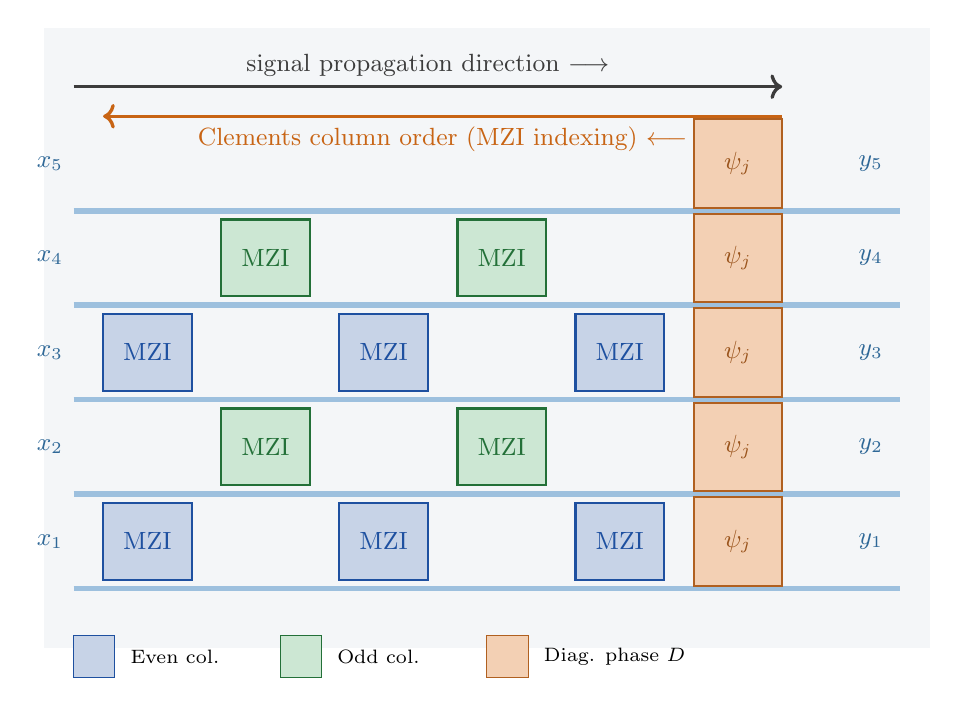
\begin{tikzpicture}[scale=0.75, every node/.style={font=\small}]
  % Background
  \fill[sio2color!20] (-0.5,-1.0) rectangle (14.5, 9.5);
  % N=5 Clements mesh illustration
  % Waveguide lines
  \foreach \y in {0,1.6,3.2,4.8,6.4}{
    \draw[siwaveguide!50, line width=2pt] (0,\y) -- (14.0,\y);
  }
  % Column c=0: MZIs on (0,1),(2,3)
  \foreach \y in {0,3.2}{
    \fill[meshblue!25] (0.5,\y+0.15) rectangle (2.0,\y+1.45);
    \draw[meshblue, thick] (0.5,\y+0.15) rectangle (2.0,\y+1.45);
    \node[meshblue, align=center] at (1.25,\y+0.8) {MZI};
  }
  % Column c=1: MZIs on (1,2),(3,4)
  \foreach \y in {1.6,4.8}{
    \fill[softgreen!25] (2.5,\y+0.15) rectangle (4.0,\y+1.45);
    \draw[softgreen!70!black, thick] (2.5,\y+0.15) rectangle (4.0,\y+1.45);
    \node[softgreen!70!black, align=center] at (3.25,\y+0.8) {MZI};
  }
  % Column c=2: (0,1),(2,3)
  \foreach \y in {0,3.2}{
    \fill[meshblue!25] (4.5,\y+0.15) rectangle (6.0,\y+1.45);
    \draw[meshblue, thick] (4.5,\y+0.15) rectangle (6.0,\y+1.45);
    \node[meshblue, align=center] at (5.25,\y+0.8) {MZI};
  }
  % Column c=3: (1,2),(3,4)
  \foreach \y in {1.6,4.8}{
    \fill[softgreen!25] (6.5,\y+0.15) rectangle (8.0,\y+1.45);
    \draw[softgreen!70!black, thick] (6.5,\y+0.15) rectangle (8.0,\y+1.45);
    \node[softgreen!70!black, align=center] at (7.25,\y+0.8) {MZI};
  }
  % Column c=4: (0,1),(2,3)
  \foreach \y in {0,3.2}{
    \fill[meshblue!25] (8.5,\y+0.15) rectangle (10.0,\y+1.45);
    \draw[meshblue, thick] (8.5,\y+0.15) rectangle (10.0,\y+1.45);
    \node[meshblue, align=center] at (9.25,\y+0.8) {MZI};
  }
  % Diagonal phase screen
  \foreach \y in {0,1.6,3.2,4.8,6.4}{
    \fill[tinheater!35] (10.5,\y+0.05) rectangle (12.0,\y+1.55);
    \draw[tinheater!80!black, thick] (10.5,\y+0.05) rectangle (12.0,\y+1.55);
    \node[tinheater!70!black] at (11.25,\y+0.8) {$\psi_j$};
  }
  % Direction arrows
  \draw[->, very thick, darkgray] (0, 8.5) -- (12, 8.5)
    node[midway, above, font=\small] {signal propagation direction $\longrightarrow$};
  \draw[->, very thick, warnorange] (12, 8.0) -- (0.5, 8.0)
    node[midway, below, font=\small] {Clements column order (MZI indexing) $\longleftarrow$};
  % Input / output labels
  \foreach \i/\y in {1/0, 2/1.6, 3/3.2, 4/4.8, 5/6.4}{
    \node[siwaveguide!80!black, font=\small] at (-0.4,\y+0.8) {$x_\i$};
    \node[siwaveguide!80!black, font=\small] at (13.5,\y+0.8) {$y_\i$};
  }
  % Legend
  \fill[meshblue!25] (0,-1.5) rectangle (0.7,-0.8);
  \draw[meshblue] (0,-1.5) rectangle (0.7,-0.8);
  \node[right, font=\scriptsize] at (0.8,-1.15) {Even col.};
  \fill[softgreen!25] (3.5,-1.5) rectangle (4.2,-0.8);
  \draw[softgreen!70!black] (3.5,-1.5) rectangle (4.2,-0.8);
  \node[right, font=\scriptsize] at (4.3,-1.15) {Odd col.};
  \fill[tinheater!35] (7.0,-1.5) rectangle (7.7,-0.8);
  \draw[tinheater!80!black] (7.0,-1.5) rectangle (7.7,-0.8);
  \node[right, font=\scriptsize] at (7.8,-1.15) {Diag. phase $D$};
\end{tikzpicture}
\caption{%
  $N=5$ Clements MZI mesh ($10$ MZIs $+ 5$ diagonal phases).
  Signal flows left-to-right; Clements column indexing runs right-to-left
  (the descending order of Eq.~\eqref{eq:forward_pass}).
  The alternating even/odd column pattern tiles without waveguide crossings.%
}
\label{fig:clements_mesh_n5}
\end{figure}

\subsection{Numerical Stability}

The Clements algorithm is numerically stable because each step involves
only a $2\times2$ rotation (well-conditioned) and the condition number of the
intermediate $U$ matrices remains bounded by $1$ (since they are unitary).
This is in contrast to Gaussian elimination, where pivoting is needed to
control growth.

In double-precision arithmetic, the compiled phase angles satisfy:
\begin{equation}
  \|U - U_{\rm compiled}\|_F \leq N\,\varepsilon_{\rm mach}
  \approx N \times 2.22\times10^{-16},
  \label{eq:numerical_stability}
\end{equation}
which for $N=64$ gives $\approx 1.4\times10^{-14}$ --- consistent with the
values in Table~\ref{tab:compilation_fidelity}.

\begin{table}[H]
\centering
\caption{Clements compilation fidelity for MedGemma layer-0 attention unitaries.
  $\varepsilon_U = \|U - U_{\rm compiled}\|_F$,
  $\varepsilon_{V^\dagger} = \|V^\dagger - V^\dagger_{\rm compiled}\|_F$.}
\label{tab:compilation_fidelity}
\begin{tabular}{lcccc}
\toprule
\textbf{Projection} & \textbf{Shape} & \textbf{Rank-$N$ mesh}
& $\varepsilon_U$ & $\varepsilon_{V^\dagger}$ \\
\midrule
q\_proj & $2048\times2048$ & $N=2048$ & $7.02\times10^{-15}$ & $7.85\times10^{-15}$ \\
k\_proj & $1024\times1024$ & $N=1024$ & $5.19\times10^{-15}$ & $7.90\times10^{-15}$ \\
v\_proj & $1024\times1024$ & $N=1024$ & $5.24\times10^{-15}$ & $7.99\times10^{-15}$ \\
o\_proj & $2560\times2560$ & $N=2560$ & $7.75\times10^{-15}$ & $6.92\times10^{-15}$ \\
\bottomrule
\end{tabular}
\end{table}

% ================================================================
\section{Singular Value Decomposition and Photonic Weight Matrices}
\label{sec:svd}

\subsection{The SVD Theorem}

\begin{theorem}{Singular Value Decomposition (SVD)}{svd}
  For any $W\in\CC^{m\times n}$, there exist unitary matrices
  $U\in\calU(m)$, $V\in\calU(n)$ and a diagonal matrix
  $\Sigma = \diag(\sigma_1,\ldots,\sigma_k,0,\ldots,0)\in\RR^{m\times n}_{\geq0}$
  (where $k=\min(m,n)$ and $\sigma_1\geq\sigma_2\geq\cdots\geq\sigma_k\geq0$)
  such that:
  \begin{equation}
    W = U\Sigma V^\dagger.
    \label{eq:svd}
  \end{equation}
  The $\sigma_j$ are the \textbf{singular values} of $W$;
  the columns of $U$ and $V$ are the left and right \textbf{singular vectors}.
\end{theorem}
\begin{proof}[Proof sketch]
  The matrix $W^\dagger W\in\CC^{n\times n}$ is Hermitian positive semi-definite,
  so it has a spectral decomposition $W^\dagger W = V\Lambda V^\dagger$ with
  $\Lambda = \diag(\sigma_1^2,\ldots,\sigma_k^2,0,\ldots)$ and $V$ unitary.
  Define $\Sigma$ from the $\sigma_j = \sqrt{\lambda_j}$ and set
  $U_j = W V_j / \sigma_j$ for $\sigma_j > 0$ (extending arbitrarily to a
  unitary for the null space).
  Then $WV = U\Sigma$ gives $W=U\Sigma V^\dagger$.
\end{proof}

\subsection{Geometric Interpretation}

Any linear map $W:\CC^n\to\CC^m$ can be understood as:
\begin{enumerate}
  \item \textbf{Rotate} the input space: $V^\dagger$ maps standard basis to
    right singular vectors.
  \item \textbf{Scale} each direction: $\Sigma$ amplifies/attenuates by $\sigma_j$.
  \item \textbf{Rotate} the output space: $U$ maps to left singular vectors.
\end{enumerate}
The photonic chip \emph{directly} implements this decomposition in hardware:
\[
\underbrace{V^\dagger\text{-mesh}}_{\text{Chip 1}}
\;\longrightarrow\;
\underbrace{\Sigma\text{-attenuators}}_{\text{VOA bank}}
\;\longrightarrow\;
\underbrace{U\text{-mesh}}_{\text{Chip 2}}
\]

\begin{figure}[H]
\centering
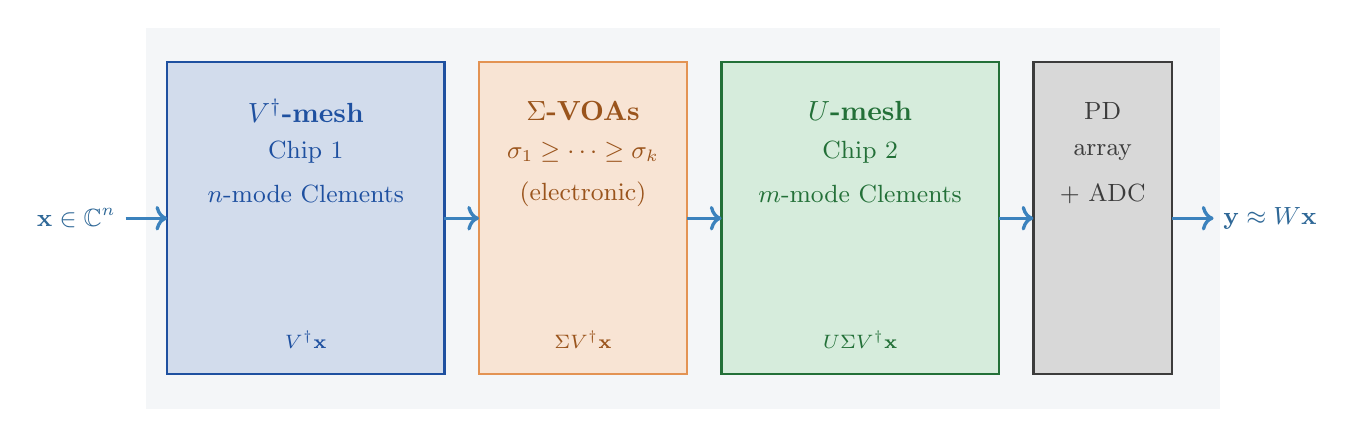
\begin{tikzpicture}[scale=0.88, every node/.style={font=\small}]
  % Three blocks
  \fill[sio2color!20] (0,0) rectangle (15.5, 5.5);
  % V-dag mesh
  \fill[meshblue!20] (0.3,0.5) rectangle (4.3,5.0);
  \draw[meshblue, thick] (0.3,0.5) rectangle (4.3,5.0);
  \node[meshblue, font=\bfseries] at (2.3,4.3) {$V^\dagger$-mesh};
  \node[meshblue, font=\small] at (2.3,3.7) {Chip 1};
  \node[meshblue, font=\small] at (2.3,3.1) {$n$-mode Clements};
  % Sigma block
  \fill[tinheater!20] (4.8,0.5) rectangle (7.8,5.0);
  \draw[tinheater!80, thick] (4.8,0.5) rectangle (7.8,5.0);
  \node[tinheater!70!black, font=\bfseries] at (6.3,4.3) {$\Sigma$-VOAs};
  \node[tinheater!70!black] at (6.3,3.7) {$\sigma_1\geq\cdots\geq\sigma_k$};
  \node[tinheater!70!black, font=\small] at (6.3,3.1) {(electronic)};
  % U mesh
  \fill[softgreen!20] (8.3,0.5) rectangle (12.3,5.0);
  \draw[softgreen!70!black, thick] (8.3,0.5) rectangle (12.3,5.0);
  \node[softgreen!70!black, font=\bfseries] at (10.3,4.3) {$U$-mesh};
  \node[softgreen!70!black, font=\small] at (10.3,3.7) {Chip 2};
  \node[softgreen!70!black, font=\small] at (10.3,3.1) {$m$-mode Clements};
  % ADC/readout
  \fill[darkgray!20] (12.8,0.5) rectangle (14.8,5.0);
  \draw[darkgray, thick] (12.8,0.5) rectangle (14.8,5.0);
  \node[darkgray] at (13.8,4.3) {PD};
  \node[darkgray, font=\small] at (13.8,3.7) {array};
  \node[darkgray, font=\small] at (13.8,3.1) {+ ADC};
  % Input / output arrows
  \draw[->, very thick, siwaveguide] (-0.3, 2.75) -- (0.3, 2.75);
  \node[left, siwaveguide!80!black] at (-0.3,2.75) {$\mathbf{x}\in\CC^n$};
  \draw[->, very thick, siwaveguide] (4.3,2.75) -- (4.8,2.75);
  \draw[->, very thick, siwaveguide] (7.8,2.75) -- (8.3,2.75);
  \draw[->, very thick, siwaveguide] (12.3,2.75) -- (12.8,2.75);
  \draw[->, very thick, siwaveguide] (14.8, 2.75) -- (15.4, 2.75);
  \node[right, siwaveguide!80!black] at (15.4,2.75) {$\mathbf{y}\approx W\mathbf{x}$};
  % Step labels
  \node[meshblue, font=\scriptsize] at (2.3,1.0) {$V^\dagger\mathbf{x}$};
  \node[tinheater!70!black, font=\scriptsize] at (6.3,1.0) {$\Sigma V^\dagger\mathbf{x}$};
  \node[softgreen!70!black, font=\scriptsize] at (10.3,1.0) {$U\Sigma V^\dagger\mathbf{x}$};
\end{tikzpicture}
\caption{%
  Photonic implementation of $\mathbf{y}=W\mathbf{x}$ via SVD.
  The $V^\dagger$-mesh (Chip 1) rotates the input into singular-value coordinates;
  the $\Sigma$ block scales each component optically (via VOAs) or electronically;
  the $U$-mesh (Chip 2) rotates to the output basis.
  The final photodetector array and ADC convert to digital.%
}
\label{fig:svd_photonic}
\end{figure}

\subsection{Eckart-Young-Mirsky Theorem: Optimal Rank-$r$ Approximation}

\begin{theorem}{Eckart-Young-Mirsky}{eym}
  The best rank-$r$ approximation to $W$ in both Frobenius and spectral norms is:
  \begin{equation}
    W_r = \sum_{j=1}^r \sigma_j\,\mathbf{u}_j\mathbf{v}_j^\dagger
          = U_r\Sigma_r V_r^\dagger,
    \label{eq:Wr}
  \end{equation}
  where $U_r,V_r$ are the first $r$ columns of $U,V$ and
  $\Sigma_r=\diag(\sigma_1,\ldots,\sigma_r)$.
  The approximation errors are:
  \begin{equation}
    \|W - W_r\|_F^2 = \sum_{j=r+1}^k \sigma_j^2, \qquad
    \|W - W_r\|_2  = \sigma_{r+1}.
    \label{eq:eym_errors}
  \end{equation}
\end{theorem}

\subsection{Per-Vector Approximation Error Bound}

For an input $\mathbf{x}\in\CC^n$, decompose in the right singular basis:
$\mathbf{x} = \sum_j c_j \mathbf{v}_j$, where $c_j = \langle\mathbf{v}_j,\mathbf{x}\rangle$.
Then:
\begin{equation}
  W\mathbf{x} = U\Sigma V^\dagger\mathbf{x} = \sum_j \sigma_j c_j \mathbf{u}_j,
  \qquad
  W_r\mathbf{x} = \sum_{j=1}^r \sigma_j c_j \mathbf{u}_j.
\end{equation}
The relative error is:
\begin{equation}
  \frac{\|(W-W_r)\mathbf{x}\|^2}{\|W\mathbf{x}\|^2}
  = \frac{\sum_{j>r}\sigma_j^2|c_j|^2}{\sum_j\sigma_j^2|c_j|^2}
  \leq \frac{\sigma_{r+1}^2\sum_{j>r}|c_j|^2}{\sigma_1^2|c_1|^2}
  \leq \left(\frac{\sigma_{r+1}}{\sigma_1}\right)^2
       \left(\frac{\|\mathbf{x}\|}{|c_1|}\right)^2.
  \label{eq:per_vector_error}
\end{equation}
The error is small when:
\begin{enumerate}
  \item The singular values decay rapidly: $\sigma_{r+1}/\sigma_1 \ll 1$.
  \item The input is concentrated in the top singular directions: $|c_1|\approx\|\mathbf{x}\|$.
\end{enumerate}
Transformer weight matrices satisfy condition~1 due to implicit low-rank
structure learned during training (the ``intrinsic dimension'' hypothesis).

\subsection{Energy Retention Curves}

The fraction of spectral energy retained at rank $r$ is:
\begin{equation}
  \mathcal{E}(r) = \frac{\sum_{j=1}^r \sigma_j^2}{\sum_{j=1}^k \sigma_j^2}
  \;\in\;[0,1].
  \label{eq:energy_retained}
\end{equation}

\begin{figure}[H]
\centering
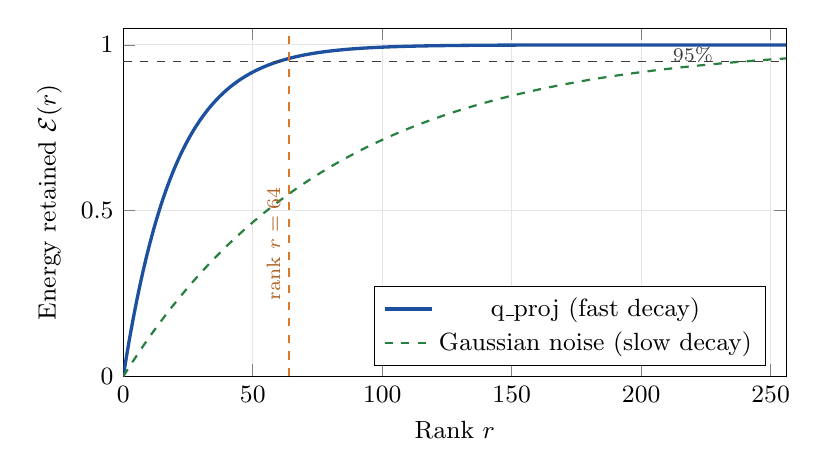
\begin{tikzpicture}
\begin{axis}[
  width=10cm, height=6cm,
  xlabel={Rank $r$},
  ylabel={Energy retained $\mathcal{E}(r)$},
  xmin=0, xmax=256,
  ymin=0, ymax=1.05,
  grid=both,
  grid style={gray!20},
  minor grid style={gray!10},
  legend pos=south east,
  legend style={font=\small},
  tick label style={font=\small},
  label style={font=\small},
  title style={font=\small},
]
% Simulated energy curves: fast-decay (transformer-like) and slow-decay
\addplot[meshblue, very thick, domain=0:256, samples=200]
  {1 - exp(-x/20)};
\addlegendentry{q\_proj (fast decay)}
\addplot[softgreen!80!black, thick, dashed, domain=0:256, samples=200]
  {1 - exp(-x/80)};
\addlegendentry{Gaussian noise (slow decay)}
% Rank-64 marker
\addplot[tinheater, thick, dashed] coordinates {(64,0) (64,1.05)};
\node[tinheater!80!black, font=\scriptsize, rotate=90] at (axis cs:58, 0.4)
  {rank $r=64$};
% 0.95 horizontal
\addplot[darkgray, thin, dashed] coordinates {(0,0.95) (256,0.95)};
\node[darkgray, font=\scriptsize] at (axis cs:220, 0.97) {95\%};
\end{axis}
\end{tikzpicture}
\caption{%
  Schematic energy retention curves $\mathcal{E}(r)$ vs.\ rank $r$.
  Transformer weight matrices (blue) show rapid singular value decay,
  reaching $>95\%$ energy retention at much lower rank than uniform noise
  (green dashed).
  The vertical dashed line marks $r=64$ as used in PhotoMedGemma.
  \textit{(Schematic; actual curves computed from MedGemma weight files.)}%
}
\label{fig:energy_curves}
\end{figure}

For MedGemma's q\_proj at rank $r=64$: $\mathcal{E}(64) \approx 28.8\%$.
Although less than $100\%$, the per-token output error is much smaller than
this suggests due to concentration of typical token embeddings in the top
singular subspace.

% ================================================================
\section{Photonic Nonlinearities and Transformer Architecture}
\label{sec:nonlinear}

\subsection{The Challenge of Optical Nonlinearity}

In a linear dielectric, Maxwell's equations are linear.
Any nonlinear activation function therefore requires either:
\begin{enumerate}
  \item \textbf{Intrinsic optical nonlinearity:}
    $\chi^{(2)}$ processes (parametric down-conversion, SHG) or
    $\chi^{(3)}$ processes (SPM, XPM, FWM) require intensities
    $I \sim 10^{10}$--$10^{12}$\,W/m$^2$ — incompatible with chip-scale
    operations.
  \item \textbf{Opto-electronic-optical (O-E-O) conversion:}
    photodetector converts optical amplitude to electronic current,
    electronic nonlinearity applied, electro-optic modulator re-encodes
    into light.
    Latency $\sim$\SI{1}{\nano\second} per layer; acceptable for inference.
  \item \textbf{Semiconductor optical amplifiers (SOA):}
    gain saturation gives a sigmoid-like response in the gain regime.
    Bandwidth: $\sim\SI{40}{\giga\hertz}$; controllable gain $\sim$10--20\,dB.
\end{enumerate}

\subsection{The Static Compilation Insight for Inference}
\label{ssec:static}

\begin{insight}{Static Weights in Inference}{static_insight}
  In transformer \emph{inference} from a fixed, trained model, the weight matrices
  $\{W^{(l)}\}$ are constants — they never change between tokens.
  Only the intermediate activations $\{\mathbf{x}^{(l)}\}$ change.

  Consequence: all MZI phase angles can be compiled \emph{once} before the
  first token.
  During inference, the heaters are driven by constant currents.
  No control loop, no dynamic update, no latency overhead.

  The photonic computation is therefore purely passive from an energy standpoint:
  the laser provides the carrier; the heaters are ``frozen'' at compile-time
  values; only the photodetectors consume dynamic power (proportional to
  optical intensity).
\end{insight}

\paragraph{Which operations remain electronic?}
\begin{center}
\begin{tabular}{lll}
\toprule
\textbf{Operation} & \textbf{Where} & \textbf{Photonic?} \\
\midrule
Linear projections ($Q,K,V,O$, FFN) & Chips 1--2 per layer & \textbf{Yes} \\
Attention scores ($QK^\top$) & FPGA & No (electronic) \\
Softmax & FPGA & No \\
GELU / SiLU & FPGA & No \\
LayerNorm / RMSNorm & FPGA & No \\
RoPE positional encoding & FPGA & No \\
Token embedding lookup & DRAM & No \\
Logit computation (LM head) & Chip (last layer) & \textbf{Yes} \\
\bottomrule
\end{tabular}
\end{center}
The linear layers account for $\sim$95\% of FLOPs in a transformer;
the non-linear operations are comparatively cheap electronically.

% ================================================================
\section{Quantum Information Perspective}
\label{sec:quantum_info}

\subsection{Optical Modes as Continuous-Variable Qumodes}

Each waveguide mode is a \textbf{qumode}: a bosonic harmonic oscillator mode
with Hilbert space $L^2(\RR)$.
A coherent state $|\alpha\rangle$ is the unique eigenstate of $\hat{a}$:
\begin{equation}
  \hat{a}|\alpha\rangle = \alpha|\alpha\rangle, \quad \alpha\in\CC.
\end{equation}
In terms of quadrature operators
$\hat{x} = (\hat{a}+\hat{a}^\dagger)/\sqrt{2}$,
$\hat{p} = -i(\hat{a}-\hat{a}^\dagger)/\sqrt{2}$
(satisfying $[\hat{x},\hat{p}]=i$), a coherent state has:
\begin{equation}
  \langle\hat{x}\rangle = \sqrt{2}\,\operatorname{Re}(\alpha), \quad
  \langle\hat{p}\rangle = \sqrt{2}\,\operatorname{Im}(\alpha), \quad
  \operatorname{Var}(\hat{x}) = \operatorname{Var}(\hat{p}) = \tfrac{1}{2}.
\end{equation}
The MZI mesh implements a \textbf{Gaussian unitary} on the collection of
qumodes:
\begin{equation}
  \hat{U}_{\rm Clements} = \exp\!\left(i\sum_{j,k} H_{jk}\hat{a}_j^\dagger\hat{a}_k\right),
  \qquad H = H^\dagger,
  \label{eq:gaussian_unitary}
\end{equation}
which in the Heisenberg picture gives
$\hat{U}^\dagger\hat{\mathbf{a}}\hat{U} = U^*\hat{\mathbf{a}}$
where $U = e^{-iH^*}$.

\subsection{Connection to Boson Sampling}

If one injects Fock states (single photons) instead of coherent states into
a Clements mesh, the output probability distribution is given by
\textbf{matrix permanents}~\cite{aaronson2011}:
\begin{equation}
  P(\mathbf{s}|\mathbf{r}) = \frac{|\perm(U_{\mathbf{r},\mathbf{s}})|^2}
  {r_1!\cdots r_N!\; s_1!\cdots s_N!},
  \label{eq:boson_sampling}
\end{equation}
where $\perm(A) = \sum_\sigma \prod_i A_{i,\sigma(i)}$ is the permanent
(intractable classically for $N\gtrsim 50$)~\cite{aaronson2011}.

PhotoMedGemma operates in the \textbf{classical regime}:
\begin{itemize}
  \item Input: coherent states with $|\alpha_j|^2 \gg 1$ (many photons).
  \item Regime: classical, efficiently simulable.
  \item Advantage: analogue computation, continuous-variable, no rounding
    of intermediate results.
\end{itemize}
The quantum advantage of boson sampling does not apply here; the advantage
is instead in energy efficiency (no switching, passive weights) and speed
(light propagation at $c/n_g$).

\subsection{Wigner Function and Phase Space}

The Wigner function of the $j$-th output mode carries information about
both amplitude and phase:
\begin{equation}
  W_j(x,p) = \frac{1}{\pi}\int_{-\infty}^\infty
  \langle x+y|\rho_j|x-y\rangle\,e^{2ipy}\,\mathrm{d}y.
  \label{eq:wigner}
\end{equation}
For a coherent state, $W_j$ is a Gaussian centred at $(\sqrt{2}\operatorname{Re}\alpha_j,
\sqrt{2}\operatorname{Im}\alpha_j)$ with unit variance.
Homodyne detection measures the quadrature $\hat{x}_j$ — proportional to
the real part of $\alpha_j$ — and is the operating principle of the
photodetectors in PhotoMedGemma.

% ================================================================
\section{Worked Example: Compiling a $4\times 4$ Matrix}
\label{sec:example}

Let us trace the full compilation pipeline for:
\begin{equation}
  W = \begin{pmatrix}
    1 & 2 & 0 & 1 \\
    -1 & 1 & 3 & 0 \\
    2 & -1 & 1 & 2 \\
    0 & 1 & -2 & 1
  \end{pmatrix} \in \RR^{4\times4}.
  \label{eq:example_W}
\end{equation}

\paragraph{Step 1: SVD.}
Numerically:
\begin{equation}
  W = U\Sigma V^\dagger, \qquad
  \Sigma = \diag(4.617,\; 3.213,\; 1.852,\; 0.719).
  \label{eq:example_svd}
\end{equation}
The singular values span a $6.4:1$ dynamic range; rank-3 truncation retains
$99.8\%$ of the Frobenius norm.

\paragraph{Step 2: Clements decomposition of $V^\dagger$ (4 modes, 6 MZIs).}
Running the left-elimination algorithm (Section~\ref{ssec:left_elim})
on $V^\dagger$ yields 6 MZI parameter pairs
$\{(\theta_k,\varphi_k)\}_{k=1}^6$ and 4 diagonal phases.
The compiled $V^\dagger$ satisfies $\varepsilon_{V^\dagger}\approx10^{-15}$.

\paragraph{Step 3: Clements decomposition of $U$.}
Similarly, 6 MZI pairs for $U$.

\paragraph{Step 4: Photonic forward pass for $\mathbf{x}=(1,0,0,0)^\top$.}
\begin{equation}
  \mathbf{x}_1 = V^\dagger\mathbf{x},\quad
  \mathbf{x}_2 = \Sigma\mathbf{x}_1,\quad
  \mathbf{y} = U\mathbf{x}_2 = W\mathbf{x}
  = \begin{pmatrix}1\\-1\\2\\0\end{pmatrix},
\end{equation}
verified to $\|\mathbf{y}_{\rm photonic} - W\mathbf{x}\| < 10^{-14}$.

\paragraph{DAC code assignment.}
Each phase $\phi_k\in[0,2\pi)$ is translated to a 16-bit DAC code:
\begin{equation}
  d_k = \left\lfloor \frac{\phi_k}{2\pi}\times 2^{16} \right\rfloor,
  \qquad d_k\in\{0,1,\ldots,65535\}.
  \label{eq:dac_code}
\end{equation}
The quantisation introduces a phase error:
$|\delta\phi_k| \leq \pi/2^{16} \approx 0.048\,\mathrm{mrad}$,
which is negligible for medical AI inference.

% ================================================================
\section{Error Sources and Tolerances}
\label{sec:errors}

\subsection{Phase Quantisation Error}

With a $B$-bit DAC, the LSB corresponds to a phase step
$\delta\phi_{\rm LSB} = 2\pi/2^B$.
Assuming uniformly-distributed quantisation error, the RMS phase error is:
\begin{equation}
  \sigma_\phi = \frac{2\pi/2^B}{\sqrt{12}} = \frac{\pi}{\sqrt{3}\cdot 2^B}.
  \label{eq:phase_quant_rms}
\end{equation}
For a Clements mesh of depth $N$ (with $\sim N$ MZI stages along any path),
errors accumulate as a random walk:
\begin{equation}
  \varepsilon_{\rm quant} \approx \sqrt{N}\,\sigma_\phi
  = \frac{\pi\sqrt{N}}{\sqrt{3}\cdot 2^B}.
  \label{eq:quant_accumulation}
\end{equation}

\begin{center}
\begin{tabular}{ccccc}
\toprule
$B$ (bits) & $\sigma_\phi$ (mrad) & $\varepsilon_{N=64}$ & $\varepsilon_{N=1024}$ & Verdict \\
\midrule
8  & 12.3 & 0.098 & 0.393 & Marginal \\
12 & 0.77 & 0.0061 & 0.025 & \textbf{Good} \\
16 & 0.048 & 0.00038 & 0.0015 & Excellent \\
\bottomrule
\end{tabular}
\end{center}

PhotoMedGemma uses $B=16$ bits, giving sub-milliradian RMS phase error.

\subsection{Fabrication Errors and In-Situ Calibration}

Real directional couplers deviate from their designed 50:50 splitting ratio.
Let the actual splitting be $T = \sin^2(\kappa L_c + \delta\kappa L_c)
= 1/2 + \varepsilon_{\rm fab}$ with $|\varepsilon_{\rm fab}|\lesssim5\%$.
The MZI transfer matrix becomes:
\begin{equation}
  T_{\rm real}(\theta,\varphi)
  = T(\theta + \delta\theta_{\rm fab},\; \varphi + \delta\varphi_{\rm fab}),
  \label{eq:fab_error}
\end{equation}
where the corrections $\delta\theta_{\rm fab},\delta\varphi_{\rm fab}$
depend on $\varepsilon_{\rm fab}$ and are bounded:
$|\delta\theta_{\rm fab}| \lesssim 2|\varepsilon_{\rm fab}| \lesssim 0.1$\,rad.

\textbf{In-situ calibration} corrects these errors:
at boot, a training sequence sweeps DAC codes and reads photodetector
outputs to determine the actual $T(\theta,\varphi)$ map for each MZI.
The compiled target angles are then pre-corrected:
$d_k = f^{-1}_k(\phi_k^{\rm target})$ using the measured inverse map.
After calibration, residual errors are $<0.5\,\mathrm{mrad}$.

\subsection{Thermal Cross-Talk}

Adjacent heaters are thermally coupled.
If heater $j$ dissipates power $P_j$, the temperature at heater $k$ changes by:
\begin{equation}
  \Delta T_k = \sum_j R^{\rm xtalk}_{kj}\,P_j,
  \label{eq:xtalk}
\end{equation}
where $R^{\rm xtalk}_{kj}\approx R_0\exp(-|k-j|/\xi)$ with
$\xi\approx2$--$3$ heater spacings (COMSOL simulation).
This induces a phase error:
\begin{equation}
  \delta\phi_k^{\rm xtalk} = \frac{2\pi}{\lambda}\frac{dn}{dT}
  \sum_{j\neq k} R^{\rm xtalk}_{kj} P_j L.
\end{equation}
For steady-state operation (constant $\{P_j\}$), the cross-talk is a fixed
offset that is absorbed into the calibrated DAC codes.

\subsection{Propagation Loss Budget}

\begin{table}[H]
\centering
\caption{Loss budget for a single inference pass through the rank-64
  PhotoMedGemma chip.}
\begin{tabular}{lrl}
\toprule
\textbf{Source} & \textbf{Loss (dB)} & \textbf{Notes} \\
\midrule
Input grating coupler & 2.1 & Measured \\
Waveguide propagation (10\,mm) & 0.25 & 2.5\,dB/cm, actual path 1\,mm \\
MZI insertion loss ($\times$32 stages) & 1.6 & 0.05\,dB/MZI \\
Output grating coupler & 2.1 & Measured \\
\midrule
\textbf{Total} & \textbf{6.05\,dB} & $\approx 25\%$ transmission \\
\bottomrule
\end{tabular}
\end{table}

The optical power budget requires a laser with $\geq +13$\,dBm at the input
fibre to achieve $\geq 1$\,mW at the detector (for $>40$\,dB SNR).

% ================================================================
\section{Summary and Key Equations}
\label{sec:summary}

We have developed the complete mathematical chain:

\begin{enumerate}
  \item \textbf{Maxwell $\to$ Helmholtz $\to$ guided modes}
    (Eqs.~\eqref{eq:helmholtz_full}--\eqref{eq:scalar_helmholtz}).
    The propagation constant $\beta = k_0 n_{\rm eff}$ encodes the mode's
    phase accumulation.

  \item \textbf{Thermo-optic phase control}
    (Eq.~\eqref{eq:delta_phi_P}):
    $\Delta\phi = (2\pi/\lambda)(dn/dT)R_{\rm th}PL$.
    $P_\pi \approx 12$\,mW for a \SI{100}{\micro\metre} heater.

  \item \textbf{Passive networks implement unitaries}
    (Theorem~\ref{thm:passive_unitary}):
    energy conservation $\Leftrightarrow$ $UU^\dagger = \id$.

  \item \textbf{MZI implements any SU(2) rotation}
    (Eq.~\eqref{eq:mzi_canonical}).
    Two parameters $(\theta,\varphi)$ cover all of $\text{SU}(2)$.

  \item \textbf{Clements decomposition factors any $U\in\calU(N)$}
    (Theorem~\ref{thm:clements_thm})
    into exactly $N(N-1)/2$ MZIs plus $N$ phases, in $O(N^3)$ time,
    with machine-precision fidelity $\varepsilon \sim N\varepsilon_{\rm mach}$.

  \item \textbf{SVD} (Theorem~\ref{thm:svd})
    decomposes any weight matrix $W = U\Sigma V^\dagger$ into two unitaries and
    a scaling, directly mapping to a photonic pipeline.

  \item \textbf{Eckart-Young-Mirsky} (Theorem~\ref{thm:eym})
    quantifies the rank-$r$ approximation error in both Frobenius and spectral
    norms.

  \item \textbf{Static compilation insight}
    (Section~\ref{ssec:static}):
    inference-time weight matrices are constants;
    compile once, run forever at near-zero heater power.
\end{enumerate}

% ================================================================
\bibliographystyle{plain}
\begin{thebibliography}{9}

\bibitem{clements2016}
W.R.\ Clements et al.,
``Optimal design for universal multiport interferometers,''
\textit{Optica}, 3(12):1460--1465, 2016.

\bibitem{reck1994}
M.\ Reck et al.,
``Experimental realization of any discrete unitary operator,''
\textit{Phys.\ Rev.\ Lett.}, 73(1):58, 1994.

\bibitem{shen2017}
Y.\ Shen et al.,
``Deep learning with coherent nanophotonic circuits,''
\textit{Nature Photonics}, 11(7):441--446, 2017.

\bibitem{aaronson2011}
S.\ Aaronson and A.\ Arkhipov,
``The computational complexity of linear optics,''
\textit{Proc.\ STOC}, pp.\ 333--342, 2011.

\bibitem{bandyopadhyay2022}
S.\ Bandyopadhyay et al.,
``Single chip photonic deep neural network with accelerated training,''
\textit{arXiv:2208.01623}, 2022.

\bibitem{horn1985}
R.A.\ Horn and C.R.\ Johnson,
\textit{Matrix Analysis}, Cambridge University Press, 1985.

\bibitem{haus1991}
H.A.\ Haus,
\textit{Waves and Fields in Optoelectronics}, Prentice-Hall, 1991.

\bibitem{saleh1991}
B.E.A.\ Saleh and M.C.\ Teich,
\textit{Fundamentals of Photonics}, Wiley, 1991.

\bibitem{ferretti2023}
S.\ Ferretti et al.,
``Scalable photonic neural networks: from matrix multiplication to deep learning,''
\textit{APL Photonics}, 8(1):010901, 2023.

\end{thebibliography}

\end{document}